\documentclass[aspectratio=169]{beamer}

% Shared preamble for Claude Code slide decks
% Usage: % Shared preamble for Claude Code slide decks
% Usage: % Shared preamble for Claude Code slide decks
% Usage: \input{preamble} after \documentclass[aspectratio=169]{beamer}

\usetheme{default}
\usecolortheme{dove}

\setbeamertemplate{navigation symbols}{}
\setbeamertemplate{footline}{%
  \hfill{\large\insertframenumber\,/\,\inserttotalframenumber}\hspace{0.8em}\vspace{0.5em}%
}

\definecolor{popblue}{RGB}{52, 101, 164}
\definecolor{sampred}{RGB}{204, 0, 0}
\definecolor{paramgreen}{RGB}{0, 140, 70}
\definecolor{lightbg}{RGB}{245, 245, 250}
\definecolor{warnred}{RGB}{180, 40, 40}
\definecolor{orange1}{RGB}{220, 120, 0}
\definecolor{violet1}{RGB}{120, 50, 160}

\setbeamercolor{frametitle}{fg=popblue}
\setbeamercolor{title}{fg=popblue}
\setbeamercolor{block title}{fg=white,bg=popblue}
\setbeamercolor{block body}{bg=lightbg}
\setbeamercolor{block title alerted}{fg=white,bg=warnred}
\setbeamercolor{block body alerted}{bg=lightbg}
\setbeamercolor{block title example}{fg=white,bg=paramgreen}
\setbeamercolor{block body example}{bg=lightbg}

\usepackage{listings}
\usepackage[T1]{fontenc}
\usepackage{hyperref}
\usepackage{tikz}
\usepackage{booktabs}
\usetikzlibrary{shapes, arrows.meta, positioning, calc}

\lstset{
  basicstyle=\ttfamily\scriptsize,
  keywordstyle=\color{popblue}\bfseries,
  stringstyle=\color{paramgreen},
  commentstyle=\color{gray},
  breaklines=true,
  frame=single,
  backgroundcolor=\color{lightbg},
  rulecolor=\color{popblue!30},
  showstringspaces=false,
  columns=fullflexible,
}
 after \documentclass[aspectratio=169]{beamer}

\usetheme{default}
\usecolortheme{dove}

\setbeamertemplate{navigation symbols}{}
\setbeamertemplate{footline}{%
  \hfill{\large\insertframenumber\,/\,\inserttotalframenumber}\hspace{0.8em}\vspace{0.5em}%
}

\definecolor{popblue}{RGB}{52, 101, 164}
\definecolor{sampred}{RGB}{204, 0, 0}
\definecolor{paramgreen}{RGB}{0, 140, 70}
\definecolor{lightbg}{RGB}{245, 245, 250}
\definecolor{warnred}{RGB}{180, 40, 40}
\definecolor{orange1}{RGB}{220, 120, 0}
\definecolor{violet1}{RGB}{120, 50, 160}

\setbeamercolor{frametitle}{fg=popblue}
\setbeamercolor{title}{fg=popblue}
\setbeamercolor{block title}{fg=white,bg=popblue}
\setbeamercolor{block body}{bg=lightbg}
\setbeamercolor{block title alerted}{fg=white,bg=warnred}
\setbeamercolor{block body alerted}{bg=lightbg}
\setbeamercolor{block title example}{fg=white,bg=paramgreen}
\setbeamercolor{block body example}{bg=lightbg}

\usepackage{listings}
\usepackage[T1]{fontenc}
\usepackage{hyperref}
\usepackage{tikz}
\usepackage{booktabs}
\usetikzlibrary{shapes, arrows.meta, positioning, calc}

\lstset{
  basicstyle=\ttfamily\scriptsize,
  keywordstyle=\color{popblue}\bfseries,
  stringstyle=\color{paramgreen},
  commentstyle=\color{gray},
  breaklines=true,
  frame=single,
  backgroundcolor=\color{lightbg},
  rulecolor=\color{popblue!30},
  showstringspaces=false,
  columns=fullflexible,
}
 after \documentclass[aspectratio=169]{beamer}

\usetheme{default}
\usecolortheme{dove}

\setbeamertemplate{navigation symbols}{}
\setbeamertemplate{footline}{%
  \hfill{\large\insertframenumber\,/\,\inserttotalframenumber}\hspace{0.8em}\vspace{0.5em}%
}

\definecolor{popblue}{RGB}{52, 101, 164}
\definecolor{sampred}{RGB}{204, 0, 0}
\definecolor{paramgreen}{RGB}{0, 140, 70}
\definecolor{lightbg}{RGB}{245, 245, 250}
\definecolor{warnred}{RGB}{180, 40, 40}
\definecolor{orange1}{RGB}{220, 120, 0}
\definecolor{violet1}{RGB}{120, 50, 160}

\setbeamercolor{frametitle}{fg=popblue}
\setbeamercolor{title}{fg=popblue}
\setbeamercolor{block title}{fg=white,bg=popblue}
\setbeamercolor{block body}{bg=lightbg}
\setbeamercolor{block title alerted}{fg=white,bg=warnred}
\setbeamercolor{block body alerted}{bg=lightbg}
\setbeamercolor{block title example}{fg=white,bg=paramgreen}
\setbeamercolor{block body example}{bg=lightbg}

\usepackage{listings}
\usepackage[T1]{fontenc}
\usepackage{hyperref}
\usepackage{tikz}
\usepackage{booktabs}
\usetikzlibrary{shapes, arrows.meta, positioning, calc}

\lstset{
  basicstyle=\ttfamily\scriptsize,
  keywordstyle=\color{popblue}\bfseries,
  stringstyle=\color{paramgreen},
  commentstyle=\color{gray},
  breaklines=true,
  frame=single,
  backgroundcolor=\color{lightbg},
  rulecolor=\color{popblue!30},
  showstringspaces=false,
  columns=fullflexible,
}


\title{Introduction to Agent Skills}
\subtitle{SKILL.md $\cdot$ Frontmatter $\cdot$ Matching $\cdot$ Sharing}
\date{}

\begin{document}

\begin{frame}
\titlepage
\end{frame}

% ──────────────────────────────────────────────
\begin{frame}{What Are Skills?}
\textbf{Skills} = reusable markdown instructions that Claude automatically applies to the right tasks at the right time.

\bigskip
\begin{block}{Key properties}
\begin{itemize}
  \item Each skill lives in a \texttt{SKILL.md} file with \textbf{name} and \textbf{description} in frontmatter
  \item Claude matches your request against skill descriptions --- activates automatically
  \item Load \emph{on demand} (unlike \texttt{CLAUDE.md} which loads every time)
\end{itemize}
\end{block}

\bigskip
\textbf{\color{orange1}Rule of thumb:} if you find yourself explaining the same thing to Claude repeatedly, that's a skill waiting to be written.

\smallskip
\textbf{Bundled skills:} \texttt{/batch}, \texttt{/simplify}, \texttt{/debug}, \texttt{/claude-api} ship with Claude Code.
\end{frame}

% ──────────────────────────────────────────────
\begin{frame}{Skills vs.\ Other Features}
\begin{table}
\centering\small
\begin{tabular}{lccc}
\textbf{Feature} & \textbf{When loaded} & \textbf{Activation} & \textbf{Scope} \\
\hline
\texttt{CLAUDE.md} & Every conversation & Always & Project-wide \\
Slash commands & On invocation & Explicit (\texttt{/cmd}) & Project/personal \\
\textbf{Skills} & On demand & \textbf{Automatic} (semantic) & Project/personal \\
Hooks & On tool use & Trigger-based & Settings file \\
MCP servers & On tool use & Tool-based & Config file \\
Subagents & On delegation & Automatic & Agent definition \\
\end{tabular}
\end{table}

\bigskip
Skills activate when Claude \emph{recognizes the situation} --- no explicit invocation needed.
\end{frame}

% ──────────────────────────────────────────────
\begin{frame}{Where Skills Live}
\begin{columns}[T]
\column{0.5\textwidth}
\textbf{\color{popblue}Personal Skills}
\begin{itemize}
  \item Location: \texttt{\textasciitilde/.claude/skills/}
  \item Follow you across \emph{all} projects
  \item Your personal coding preferences
\end{itemize}

\column{0.5\textwidth}
\textbf{\color{paramgreen}Project Skills}
\begin{itemize}
  \item Location: \texttt{.claude/skills/}
  \item Shared with anyone who clones the repo
  \item Team conventions \& workflows
\end{itemize}
\end{columns}

\bigskip
\textbf{Priority hierarchy} (name conflicts):
\begin{center}
\large
Enterprise $\to$ Personal $\to$ Project $\to$ Plugins
\end{center}
\end{frame}

% ──────────────────────────────────────────────
\begin{frame}[fragile]{Creating Your First Skill}
\textbf{Directory structure:}
\begin{lstlisting}
~/.claude/skills/
  pr-description/
    SKILL.md
\end{lstlisting}

\textbf{SKILL.md with frontmatter:}
\begin{lstlisting}[]
---
name: pr-description
description: >
  Generate a pull request description from the
  current branch's changes. Summarize what changed,
  why, and any testing notes.
---

When asked to create a PR description:
1. Run `git diff main...HEAD` to see all changes
2. Summarize the purpose of the changes
3. List key files modified
4. Note any breaking changes or migration steps
5. Suggest reviewers based on file ownership
\end{lstlisting}
\end{frame}

% ──────────────────────────────────────────────
\begin{frame}{How Skill Matching Works}
\begin{center}
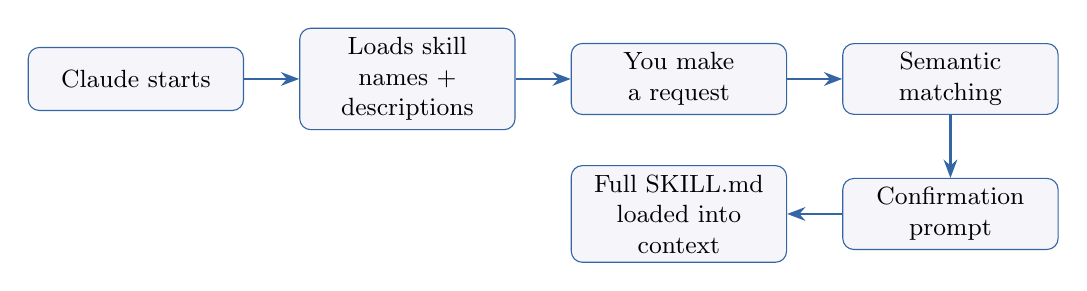
\begin{tikzpicture}[
  node distance=0.6cm and 0.7cm,
  box/.style={rectangle, rounded corners, draw=popblue, fill=lightbg,
              text width=2.5cm, minimum height=0.8cm, align=center, font=\small},
  arr/.style={-Stealth, thick, popblue}
]
  \node[box] (start) {Claude starts};
  \node[box, right=of start] (load) {Loads skill\\names + descriptions};
  \node[box, right=of load] (req) {You make\\a request};
  \node[box, right=of req] (match) {Semantic\\matching};
  \node[box, below=0.8cm of match] (prompt) {Confirmation\\prompt};
  \node[box, left=of prompt] (full) {Full SKILL.md\\loaded into context};
  \draw[arr] (start) -- (load);
  \draw[arr] (load) -- (req);
  \draw[arr] (req) -- (match);
  \draw[arr] (match) -- (prompt);
  \draw[arr] (prompt) -- (full);
\end{tikzpicture}
\end{center}

\bigskip
\begin{alertblock}{Important}
Only names and descriptions are loaded at startup. The full skill body is loaded \emph{only after confirmation} --- keeps context window lean.
\end{alertblock}
\end{frame}

% ──────────────────────────────────────────────
\begin{frame}[fragile]{Configuration \& Multi-File Skills}
\textbf{Frontmatter options:}
\begin{lstlisting}[]
---
name: deploy-checker
description: Validate deployment readiness
allowed-tools:
  - Bash
  - Read
model: sonnet
context: fork          # run in isolated subagent
user-invocable: true   # show in / menu
---
\end{lstlisting}
\smallskip
\textbf{Progressive disclosure} --- multi-file skills:
\begin{lstlisting}
.claude/skills/deploy-checker/
  SKILL.md       # main entry point
  scripts/       # shell scripts, Python, etc.
  templates/     # report templates
\end{lstlisting}

\footnotesize
Skills can reference supporting files, scripts, and templates. Dynamic context injection available at load time.
\end{frame}

% ──────────────────────────────────────────────
\begin{frame}{Sharing Skills}
\begin{columns}[T]
\column{0.5\textwidth}
\textbf{\color{popblue}Via Repository}
\begin{itemize}
  \item Commit \texttt{.claude/skills/} to git
  \item Team members get skills on clone
  \item Version-controlled conventions
\end{itemize}

\bigskip
\textbf{\color{violet1}Via Plugins}
\begin{itemize}
  \item Installable skill packages (834+ available)
  \item Cross-project reuse
  \item Agent Skills open standard (\texttt{agentskills.io})
\end{itemize}

\column{0.5\textwidth}
\textbf{\color{paramgreen}Enterprise Managed}
\begin{itemize}
  \item Org-wide skill deployment
  \item Highest priority in hierarchy
  \item Enforce standards at scale
\end{itemize}

\bigskip
\textbf{\color{orange1}Skills + Subagents}
\begin{itemize}
  \item Skills can invoke subagents
  \item Combine instructions with\\specialized agents
  \item Powerful composition pattern
\end{itemize}
\end{columns}
\end{frame}

% ──────────────────────────────────────────────
\begin{frame}{Troubleshooting Skills}
\begin{alertblock}{Common Issues}
\begin{enumerate}
  \item \textbf{Skill doesn't trigger} --- description too vague; make it specific and action-oriented
  \item \textbf{Wrong skill triggers} --- descriptions overlap; differentiate with distinct verbs/contexts
  \item \textbf{Skill not loading} --- check file path, frontmatter YAML syntax, restart Claude
  \item \textbf{Priority conflict} --- remember: Enterprise $>$ Personal $>$ Project $>$ Plugins
  \item \textbf{Runtime errors} --- test skill instructions manually first
\end{enumerate}
\end{alertblock}

\bigskip
\begin{exampleblock}{Tip: Verify skill loading}
Restart Claude Code and confirm your skill appears in the skill list. If it doesn't, check the file path and YAML frontmatter syntax.
\end{exampleblock}
\end{frame}

% ──────────────────────────────────────────────
\begin{frame}{Summary}
\begin{block}{Key Takeaways}
\begin{itemize}
  \item Skills = \textbf{reusable instructions} that activate automatically via semantic matching
  \item Frontmatter: \texttt{name}, \texttt{description}, \texttt{allowed-tools}, \texttt{model}, \texttt{context}, \texttt{user-invocable}
  \item Personal (\texttt{\textasciitilde/.claude/skills/}) vs.\ Project (\texttt{.claude/skills/})
  \item Write specific descriptions --- they are the matching key
  \item Share via git, plugins, or enterprise managed settings
  \item Multi-file skills with progressive disclosure and dynamic context injection
\end{itemize}
\end{block}

\vfill
\centering
\Large\color{popblue} Questions?
\end{frame}

\end{document}
